\chapter{Analysis and Results} \label{chapter: Analysis&Results}
This chapter first provides information about the analyses of the quantitative data and their subsequent results \ref{Sec: Quant analysis}, followed by reasoning of the type of analysis used for the open-text qualitative responses \ref{Sec: Qual Analysis}, their implementation and results to provide a concise and clear understanding of the processes. Additionally, the methods used to analyze the DPDPA related questions were discussed in \ref{sec:DPDPA analysis}.

\section{Quantitative Analysis} \label{Sec: Quant analysis}

As we have seen in chapter \ref{Sec:Privacy Notice}, the survey primarily consists of Likert-based questions, which were in the form of 5-point (Sensitivity scale and Agreement scale) or 7-point (Agreement scale) scales depending on the section in which they were used. Participant responses to these questions were initially checked for completeness and then coded to each scale's numeric equivalent values of 1-5 or 1-7 to ensure ease in calculations. Likert responses are considered to be ordinal in nature, due to the presence of ordered data but without any clear intervals between them which meant that non-parametric tests were to be used. To ensure demographics weren't overlapping with each other when comparing their effects on various results, cross-tabs were calculated and it was found that ~77\% of the respondents with Technical background were below the age of 35. For this reason only one of the two was considered while looking at their effects, as effect isolation would not be possible due to the very high overlap\footnote{While primary Regression analysis only considers Gender and Field of work as the indicators, Age was also considered as an indicator and the subsequent effects were calculated to ensure robustness. These Results can be found in the Appendix}. Age and Gender cross-tab was also checked, with \textit{Non-binary} and \textit{prefer not to say} options being omitted from further comparative effect analysis due to their low count. It was seen that there were only 64\% of the men were having technical backgrounds and the lower overlap meant that the effects could be looked at both as bivariates and individual indicators while isolating one another. Additionally, basic descriptive statistics like Mean\footnote{Mean was calculated just for showcasing the rough response split which was also visible using the frequency distribution table, and was not used for any further comparisons}, Median, Variance, Skew for each of the sections was calculated along with the frequency distributions for easier plotting of the distribution of the participants' responses.

\subsection{IUIPC Subscales} \label{Subsec: IUIPC analysis}
The Internet Users' Information Privacy Concern scale was adapted (See \ref{Adapted_Survey}) to best suite the perspectives of the local demographics, ensuring that the scale retained its legibility despite the change in context. A high ceiling effect was found in the responses which can be seen in the frequency distribution table (See figure \ref{fig:IUIPC Frequency}).

\begin{figure}[htbp]
    \centering
    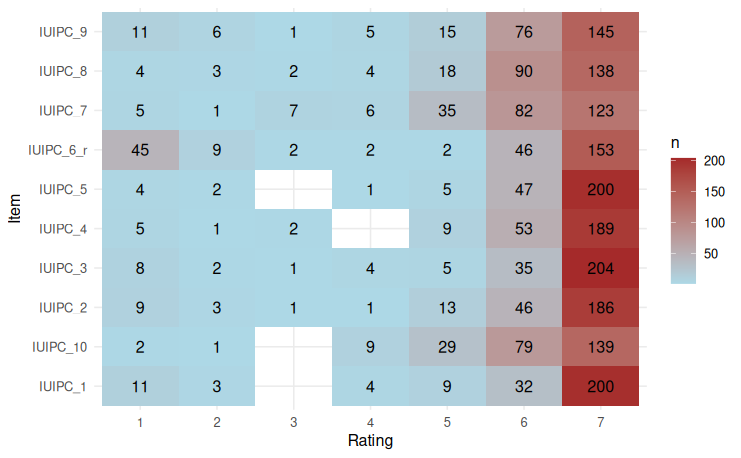
\includegraphics[width=0.9\linewidth]{Plots/IUIPC_frequency.png}
    \caption{Frequency distribution of respondents for Section - 1}
    \label{fig:IUIPC Frequency}
\end{figure}  

Since Pearson's correlation assumes normality and only looks for linear relationships, Spearman's correlations were calculated to check how the items actually correlated with items from the same and other sub-scales. The collection and control items correlated well within their own sub-scale and poorly with the others. However, awareness items showed weak correlation with each other, primarily due to some participants misreading the reverse-keyed statement. These correlations can be seen in \ref{fig:IUIPC correlations}. In order to calculate the internal consistency of each sub-scale , Cronbach's Alpha was calculated. In order to understand the complete picture of each sub-scale, their r.drop values, Feldt CI intervals and `reliability if an item is dropped' were also calculated. This sub-scale's $\alpha$ was 0.22 with broad Feldt Confidence Intervals at 0.04 - 0.37. Additionally, the r.drop value for Item 6 was 0.0024, and the $\alpha$ of the sub-scale shot back up to 0.777 if this item was removed. These values confirmed the poor correlation for the awareness sub-scale and ensured that it couldn't be used for further calculations. Since it is not recommended to have scales with only two items in it, the decision to further not consider this sub-scale was made. Control and Collection sub-scales had good $\alpha$ values of 0.76 and 0.77 respectively. Alpha statistics for all the three sub-scales are available in the Appendix. \ref{control_IUIPC} \ref{collection_IUIPC} \ref{awareness_IUIPC}  

\begin{figure}[htbp]
    \centering
    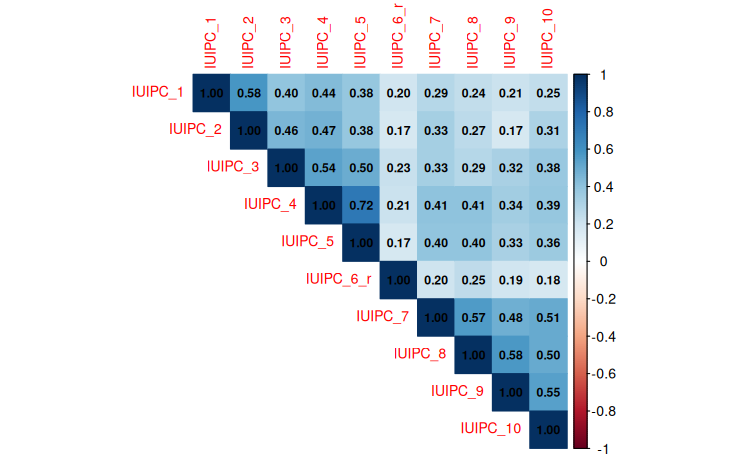
\includegraphics[width=1.0\linewidth]{Plots/IUIPC_correlation.png}
    \caption{Spearman's item to item correlation (Item 6 has very weak correlations with item 4 (0.21) and item 5 (0.17))}
    \label{fig:IUIPC correlations}
\end{figure}

\subsection{Personal Data Sensitivity} \label{Subsec: PD analysis}

Along with the common descriptive statistics, Inter Quartile Range (IQR) was also calculated to better explain the spread of the data based on the percentile values. These values can be seen in the table \ref{tab:privacy_statistics}.


\begin{table}[h]
\centering
\caption{Statistical Summary of Privacy Sensitivity Ratings}
\label{tab:privacy_statistics}
\begin{tabular}{lrrrr}
\toprule
\textbf{Name} & \textbf{Mean} & \textbf{Median} & \textbf{SD} & \textbf{IQR} \\
\midrule
Name & 2.880309 & 3 & 1.3601322 & 2.0 \\
Gender-sensitivity & 2.297297 & 2 & 1.1912278 & 2.0 \\
Phone number & 4.247104 & 5 & 0.9688668 & 1.0 \\
Address & 4.444015 & 5 & 0.8847069 & 1.0 \\
Sexual orientation & 3.316602 & 3 & 1.3554921 & 1.5 \\
Caste & 3.420849 & 3 & 1.3908998 & 2.5 \\
Ethnicity & 3.193050 & 3 & 1.3241166 & 2.0 \\
Religion & 3.254826 & 3 & 1.3881858 & 3.0 \\
Credit/Debit card details & 4.915058 & 5 & 0.3302059 & 0.0 \\
Bank Account details & 4.926641 & 5 & 0.3387516 & 0.0 \\
Tax information & 4.687259 & 5 & 0.7143815 & 0.0 \\
Aadhaar details & 4.683398 & 5 & 0.7314598 & 0.0 \\
Passport details & 4.702703 & 5 & 0.6879587 & 0.0 \\
PAN details & 4.702703 & 5 & 0.6532807 & 0.0 \\
Photographs & 4.397683 & 5 & 0.9108277 & 1.0 \\
Fingerprints/Biometric information & 4.926641 & 5 & 0.3150377 & 0.0 \\
IP addresses & 4.528958 & 5 & 0.8177603 & 1.0 \\
Device details & 4.328185 & 5 & 0.9257393 & 1.0 \\
Browser history & 4.432432 & 5 & 0.8296062 & 1.0 \\
GPS location & 4.602317 & 5 & 0.7314598 & 1.0 \\
Email addresses & 3.660232 & 4 & 1.2264848 & 2.0 \\
Passwords & 4.903475 & 5 & 0.3966276 & 0.0 \\
Medical records and history & 4.382239 & 5 & 0.8829968 & 1.0 \\
\bottomrule

\end{tabular}
\end{table}

A Friedman rank-sum test was conducted to assess differences in sensitivity ratings across the 23 privacy categories. The test indicated significant differences among categories, $\chi^2(22) = 2564.3$, p < .001. Kendall's coefficient \footnote{Kendall's W measures the effect size by normalizing the value of Friedman's between 0 (no agreement) to 1 (complete agreement)} revealed moderate inter-rater agreement, W = 0.45, $\chi^2(22) = 2564.3$, p < .001. This meant that while participants showed consensus on rankings, items varied individually in terms of their distribution. This is also in alignment with the frequency distribution seen in Figure \ref{fig:Frequency sensitivity}. 

\begin{figure}[htbp]
    \centering
    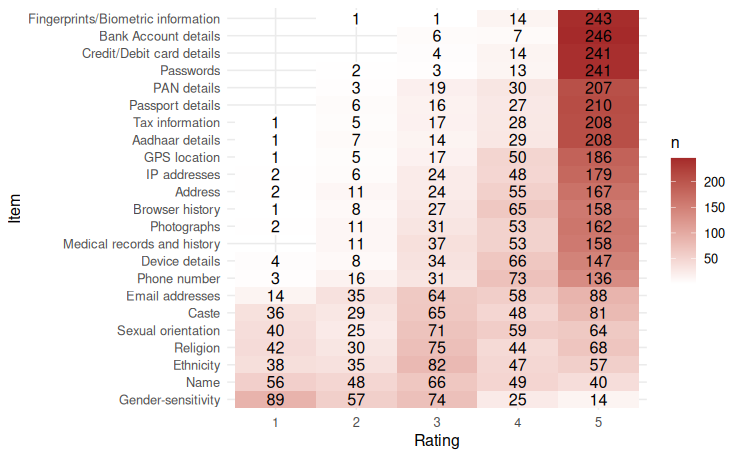
\includegraphics[width=1.0\linewidth]{Plots/Sensitivity_frequency.png}
    \caption{Frequency distribution of the Personal data items (n=259)}
    \label{fig:Frequency sensitivity}
\end{figure}

Despite these personal data items initially being considered as a battery, they were clustered to see if there was any possible correlation between the clusters and other sub-scales in the survey. They were grouped together based on how they clustered with one another in their frequency distribution and clustering from previous works. The following groupings were considered:

\begin{itemize}
    \item Demographics : Name, Gender, Sexual orientation, Caste, Ethnicity, Religion, Address, Phone number
    \item Financial : Credit/Debit card details, Bank Account details, Tax information
    \item Identity : Aadhaar details, PAN details, Passport details, Photographs, Fingerprints/Biometric information
    \item Technical : IP addresses, Device details, Browser history, GPS location, Email addresses, Passwords
    \item Medical : Medical records and history
\end{itemize}

Upon checking the internal validity using Spearman's correlations and Cronbach's $\alpha$ for each of these groups, it was observed that some of the items ranked very poorly against the others in their respective groups  \ref{fig:corr_demographics}, \ref{fig:corr_financial}, \ref{fig:corr_identity}, and \ref{fig:corr_technical}.  Additionally, Table \ref{tab:Personal data_clustered_alpha} shows that the $\alpha$ values changed substantially when the said items are omitted from the clusters. Therefore in order to ensure validity, \textit{Passwords}, \textit{Photographs}, and \textit{Fingerprints/Biometric information} were considered as individual items and \textit{Phone number} and \textit{Address} were clubbed together as contact group since they correlated well. This segregation ensured ease of comparison and validity in the process while staying true to the correlations.

\begin{table}[htbp]
    \centering
    \begin{tabular}{|c|c|c|c|l|l|l|}\hline
 & \multicolumn{3}{|c|}{Clustered} & \multicolumn{3}{|c|}{Post - Changes}\\\hline
         &  \textbf{Lower}& \textbf{Alpha}& \textbf{Upper} & \textbf{Lower}& \textbf{Alpha}& \textbf{Upper} \\\hline
         Demographics&  0.81&  0.84& 0.87 & 0.82& 0.85& 0.88\\\hline
         Financial&  0.59&  0.67& 0.73 & 0.59& 0.67& 0.73\\\hline
         Identity&  0.62&  0.69& 0.74 & 0.75& 0.79& 0.83\\\hline
         Technical& 0.61& 0.67& 0.73 & 0.62& 0.69& 0.74\\\hline\hline
    \end{tabular}
    \caption{Alpha with 95\% Feldt confidence intervals for the different Personal data clusters and the difference in values post the removal of low-correlating items from the clusters}
    \label{tab:Personal data_clustered_alpha}
\end{table}

To examine the relationships between sensitivities of these groups against the collection and control sub-scales of IUIPC and the \textit{perceived control} value of each participant, Spearman's rank order corelation was calculated. These 27 correlations across the 3 constructs and nine groups (demographic, financial, identity, technical, contact, photographs, fingerprints, passwords, medical) was denoted by Spearman's $\rho$. To control for Type I error inflation from multiple hypothesis testing, p-values were adjusted using the Holm-Bonferroni sequential correction method, which is more powerful than traditional Bonferroni adjustment while maintaining family-wise error rate control. Statistical significance was evaluated at $\alpha$ = 0.05 following Holm-adjustment.

\subsubsection{Correlation with IUIPC Collection}
All nine data sensitivity categories showed statistically significant positive associations with IUIPC Collection concerns (all p\_holm < 0.05), ranging from small effects (passwords: $\rho$ = 0.142) to medium effects (technical data: $\rho$ = 0.321; identity documents: $\rho$ = 0.307).

\subsubsection{Correlation with IUIPC Control}

Similarly, eight of nine categories showed significant positive correlations with IUIPC Control, with the notable exception of demographic data ($\rho$ = 0.077, p\_holm = 0.215). The strongest association was observed for identity documents ($\rho$ = 0.373), followed by medical records ($\rho$ = 0.305).

\subsubsection{Correlation with Perceived control}

In contrast to the other two constructs, \textit{Perceived control} demonstrated predominantly negative (inverse) relationships with data sensitivity. Two categories showed significant negative correlations: identity ($\rho$ = -0.203, p\_holm = 0.009) and medical ($\rho$ = -0.194, p\_holm = 0.014). Seven of nine associations were non-significant, with correlations near zero (For example, technical: $\rho$ = -0.019; demographic: $\rho$ = -0.023). 

However, the ceiling effect seen in the IUIPC subscales \ref{fig:IUIPC Frequency} and in several personal data items including \textit{Medical records and history}, \textit{Passport details}, \textit{Passwords}, and \textit{Aadhaar details} \ref{fig:Frequency sensitivity} is a major caveat to be remembered while understanding these values. Coincidentally, the group of personal data items which has a substantial variance across participants is \textit{demographics}, which showcased no significant correlations or only a very small effect size ($\rho$ = 0.184) across the three constructs. The complete correlation information can be seen in the figure \ref{fig:Sensitivity correlation}

\begin{figure}[htbp]
    \centering
    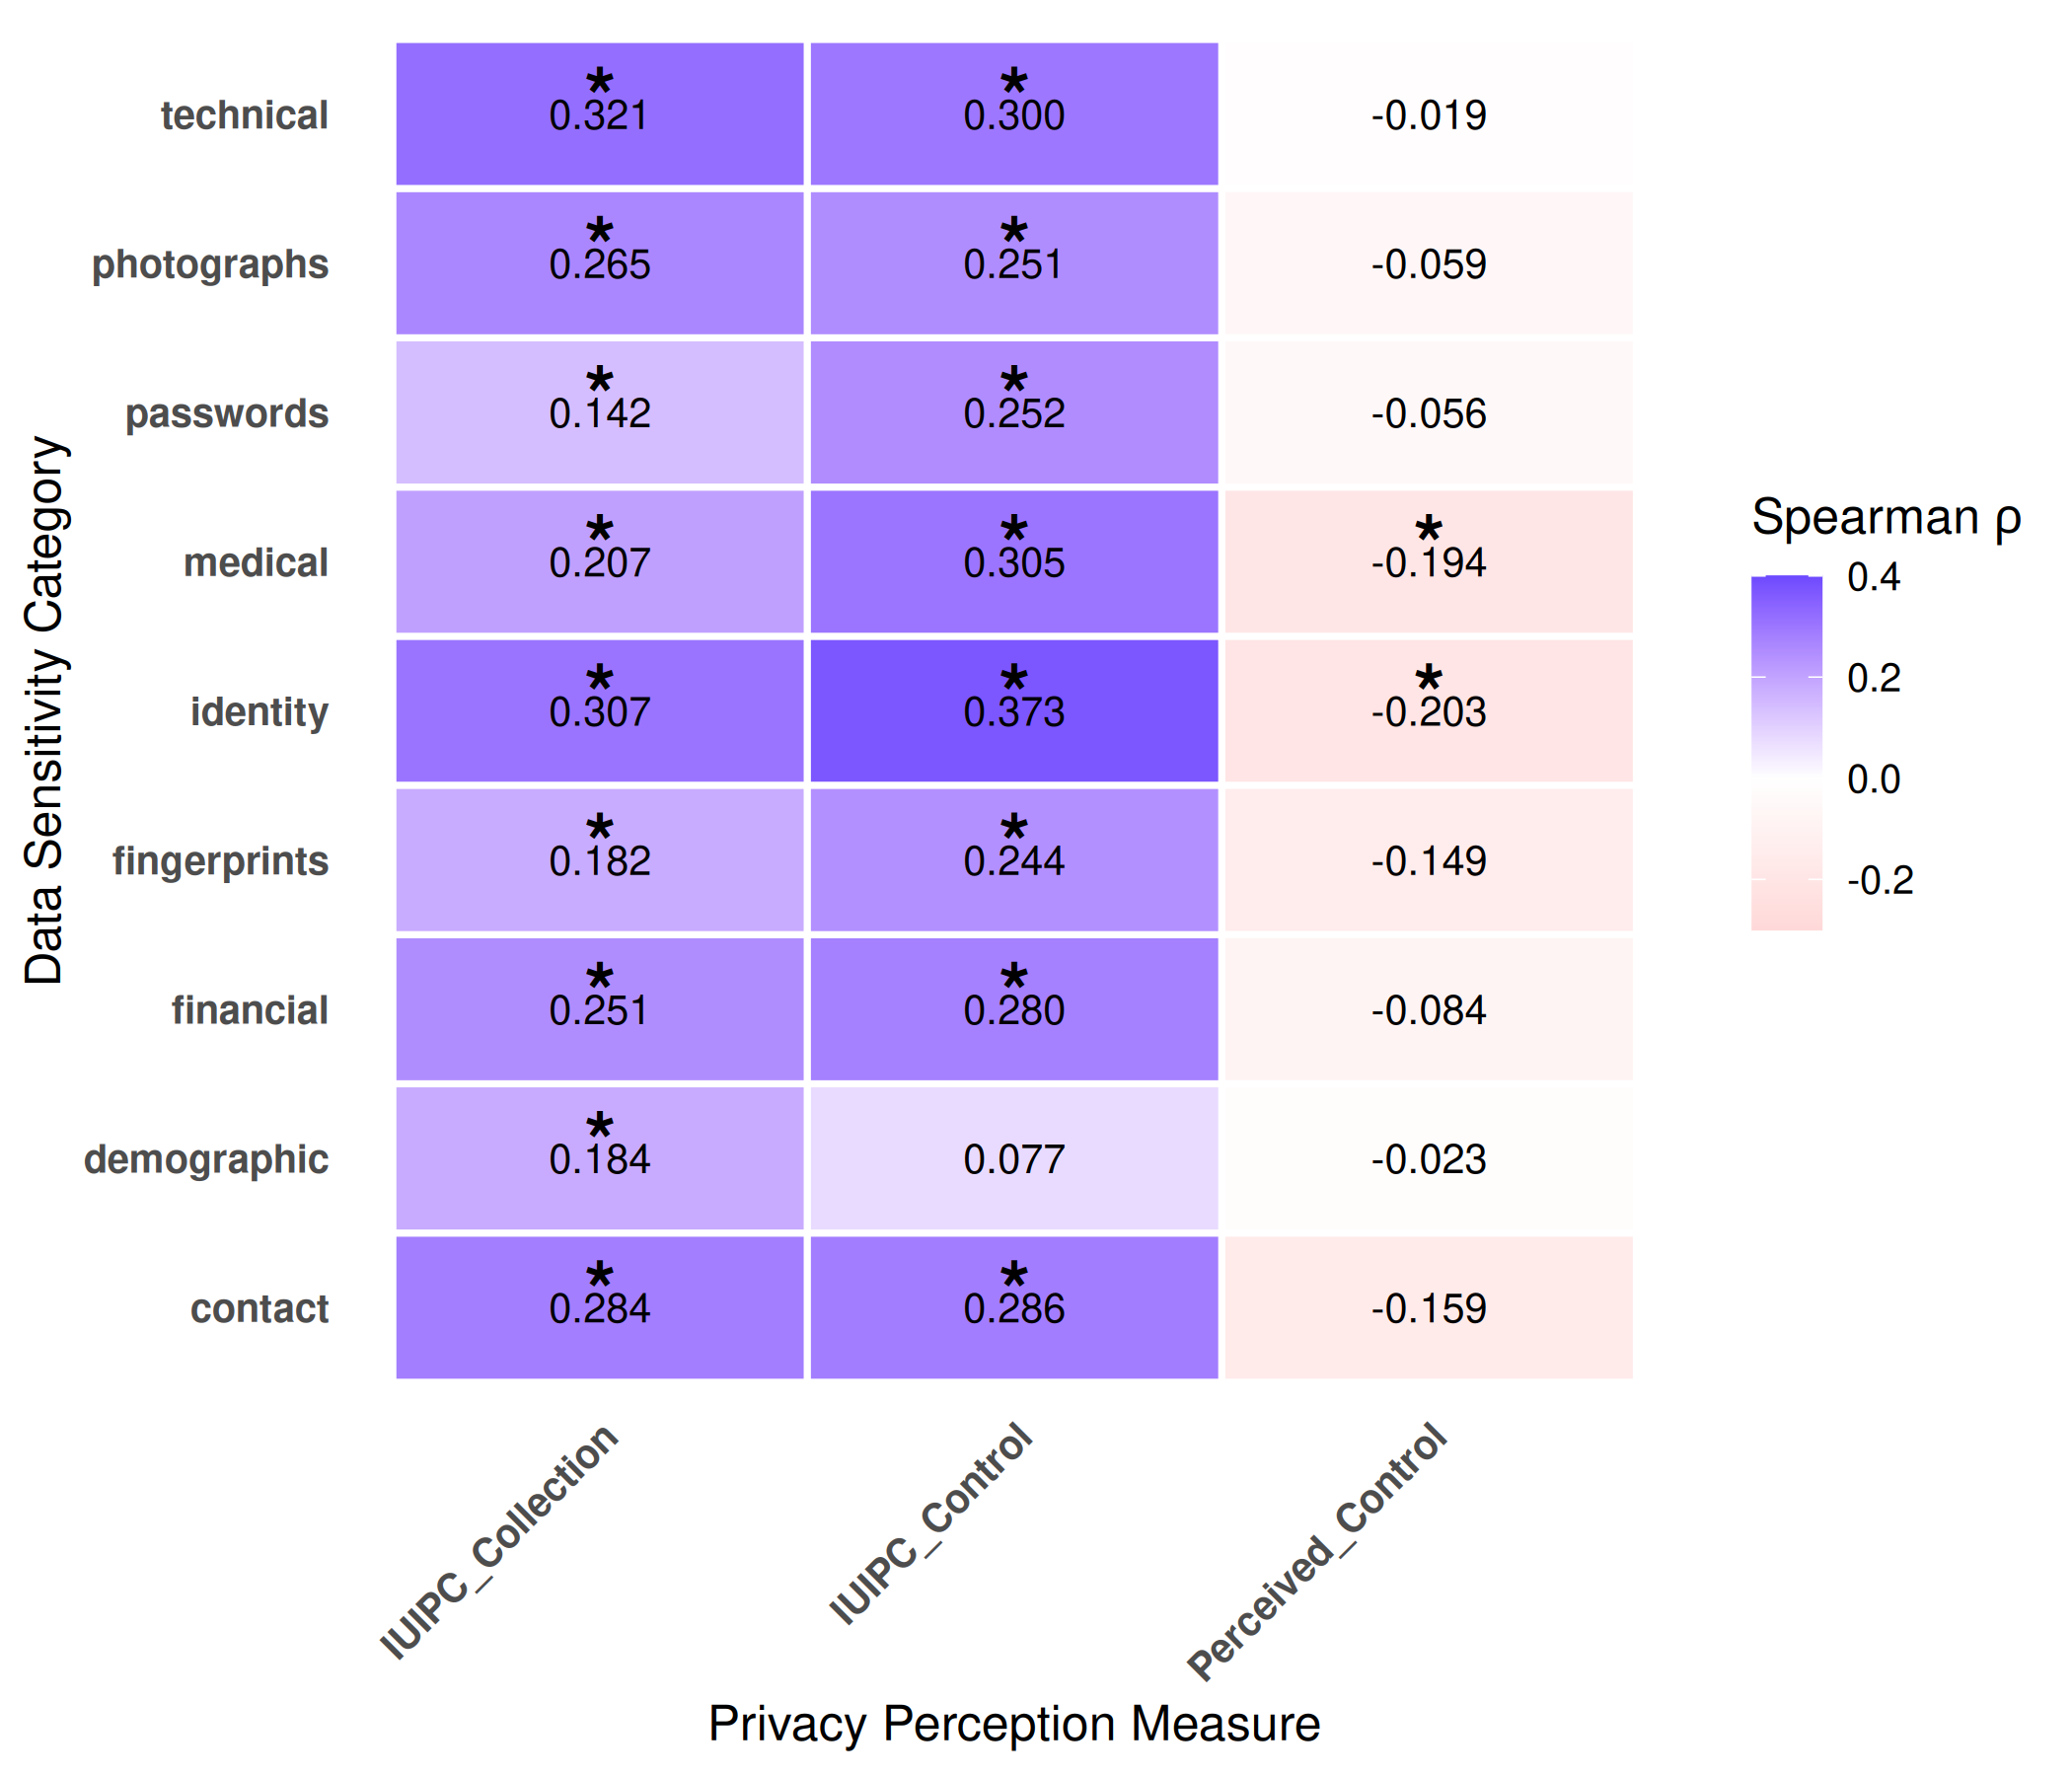
\includegraphics[width=1.0\linewidth]{Plots/Sensitivity_correlation_heatmap.png}
    \caption{Spearman correlation coefficients between nine data sensitivity categories 
and three privacy perception measures. Purple shading indicates positive correlations; 
pink shading indicates negative correlations. Asterisks denote statistical significance 
following Holm-Bonferroni correction (p < 0.05). Technical data and identity documents 
show the strongest positive associations with collection and control concerns, whereas 
perceived control demonstrates predominantly negative (non-significant) relationships.}
    \label{fig:Sensitivity correlation}
\end{figure}

\subsection{Control over processing} \label{Subsec: Perceived control analysis}
The six items in this section had a noticeably equal and uniform distribution in the responses,inferred from the descriptive statistics \ref{tab:perceived_control_descriptive} and the frequency distribution \ref{fig:Perceived_control_distribution}. This prompted the need to calculate Spearman's inter-item correlation along with Cronbach's $\alpha$ to validate the use of an aggregated value instead of using all the items. The items showed a medium-high correlation with one another as seen in the figure \ref{fig:Percevied_control_correlation} .  Combined with the high $\alpha$ value of 0.86 and Feldt CI range of 0.84 - 0.89, this meant that the scores of these 6 items, could be replaced by a singular aggregate value for each respondent. This singular value is termed as the \textit{Perceived Control} of the users, since these questions explicitly try to understand the users' perceptions of how much control they believe to be having over their Personal Data's processing and the laws which could help them in such situations.

In order to better understand how the user valued the general control over their personal data and their perceived control of its processing practices, IUIPC's control sub-scale scores of every respondent were aggregated and compared against their \textit{Perceived Control} values. Spearman rank-order correlation was conducted to examine this relationship. A weak, statistically significant negative correlation was found, $\rho$ = -0.18, p = .004, indicating that as IUIPC control increases, perceived control tended to decreases. However, it is to be noted that the previously observed pronounced ceiling effect in IUIPC control plays a significant role in ensuring this result cannot be considered at face-value due to the lack of variance. 

\begin{table}[htbp]
    \centering
    \begin{tabular}{|c|c|c|c|}\hline
         \textbf{Item}&  \textbf{Mean}& \textbf{ Median}& \textbf{SD}\\\hline
         Control 1&  2.92&  3& 1.41\\\hline
         Control 2&  3.22&  3& 1.40\\\hline
         Control 3&  2.54&  2& 1.39\\\hline
         Control 4&  2.73&  3& 1.34\\\hline
         Control 5&  3.26&  3& 1.24\\\hline
         Control 6&  2.84&  3& 1.31\\\hline
    \end{tabular}
    \caption{Descriptive Statistics of respondent's control over their processing}
    \label{tab:perceived_control_descriptive}
\end{table}

\begin{figure}[htbp]
    \centering
    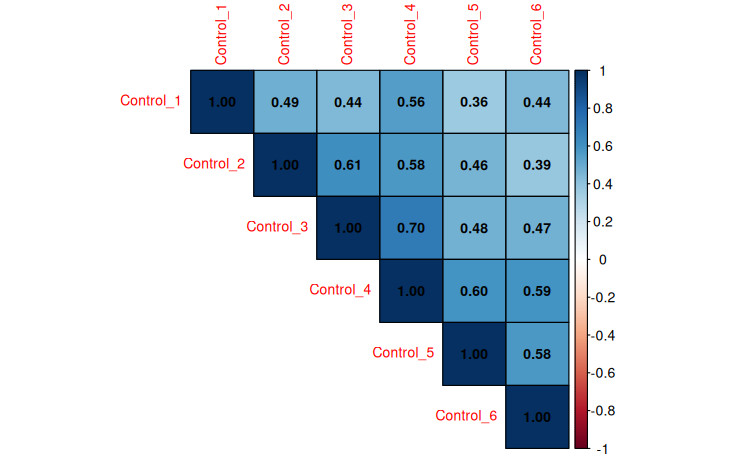
\includegraphics[width=0.9\linewidth]{Plots/Perceived_control_correlations.png}
    \caption{Spearman's correlation matrix of the six control items, with a medium-high correlation overall ranging from 0.36 - 0.70}
    \label{fig:Percevied_control_correlation}
\end{figure}


\begin{figure}[htbp]
    \centering
    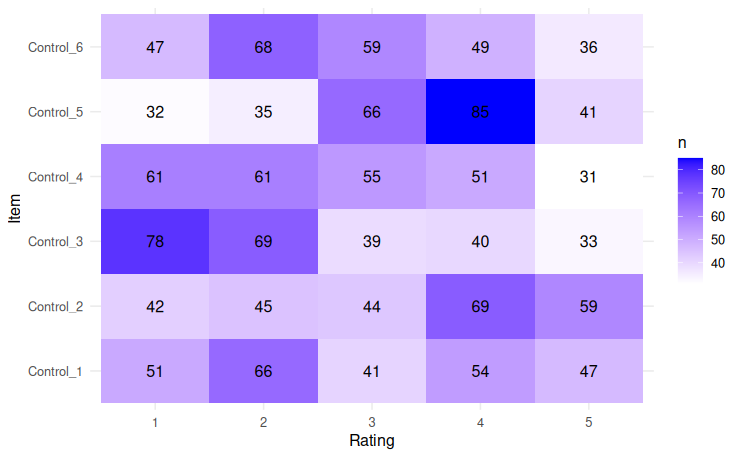
\includegraphics[width=1.0\linewidth]{Plots/Perceived control distribution.png}
    \caption{Frequency distribution of participants related to their control over the processing of their Personal Data}
    \label{fig:Perceived_control_distribution}
\end{figure}

\subsubsection{Demographic Effects} \label{subsubsub:demo effects}

To check if the demographics of the respondents, specifically their \textit{Gender} and \textit{Field of work} showed any variance on personal data sensitivity, Mann Whitney U tests were conducted comparing women versus men and technical versus non-technical sacross the 22 categories. Since the number of sensitivity items meant that the same data had to be run across 23 tests, controlling Type I error inflation from multiple hypothesis testing, p\_values were therefore adjusted using the Holm-Bonferroni sequential correction method, which is more powerful than traditional Bonferroni adjustment while maintaining family-wise error rate control.  Additionally, effect sizes were also calculated using r = Z/$\sqrt{N}$ %(Cohen,88) 
to understand how much impact the significant values are having on each item. As shown in Figure \ref{fig:Sensitivity MWU}, both \textit{Gender} and \textit{Field of work} yielded no statistically significant effects after Holm adjustment. Ordinal logistic regression models were also estimated to understand the isolated effects of the demographics, however, none of their coefficients achieved statistical significance after Holm correction (all p\_holm > 0.12).    

\begin{figure} [htbp]
    \centering
    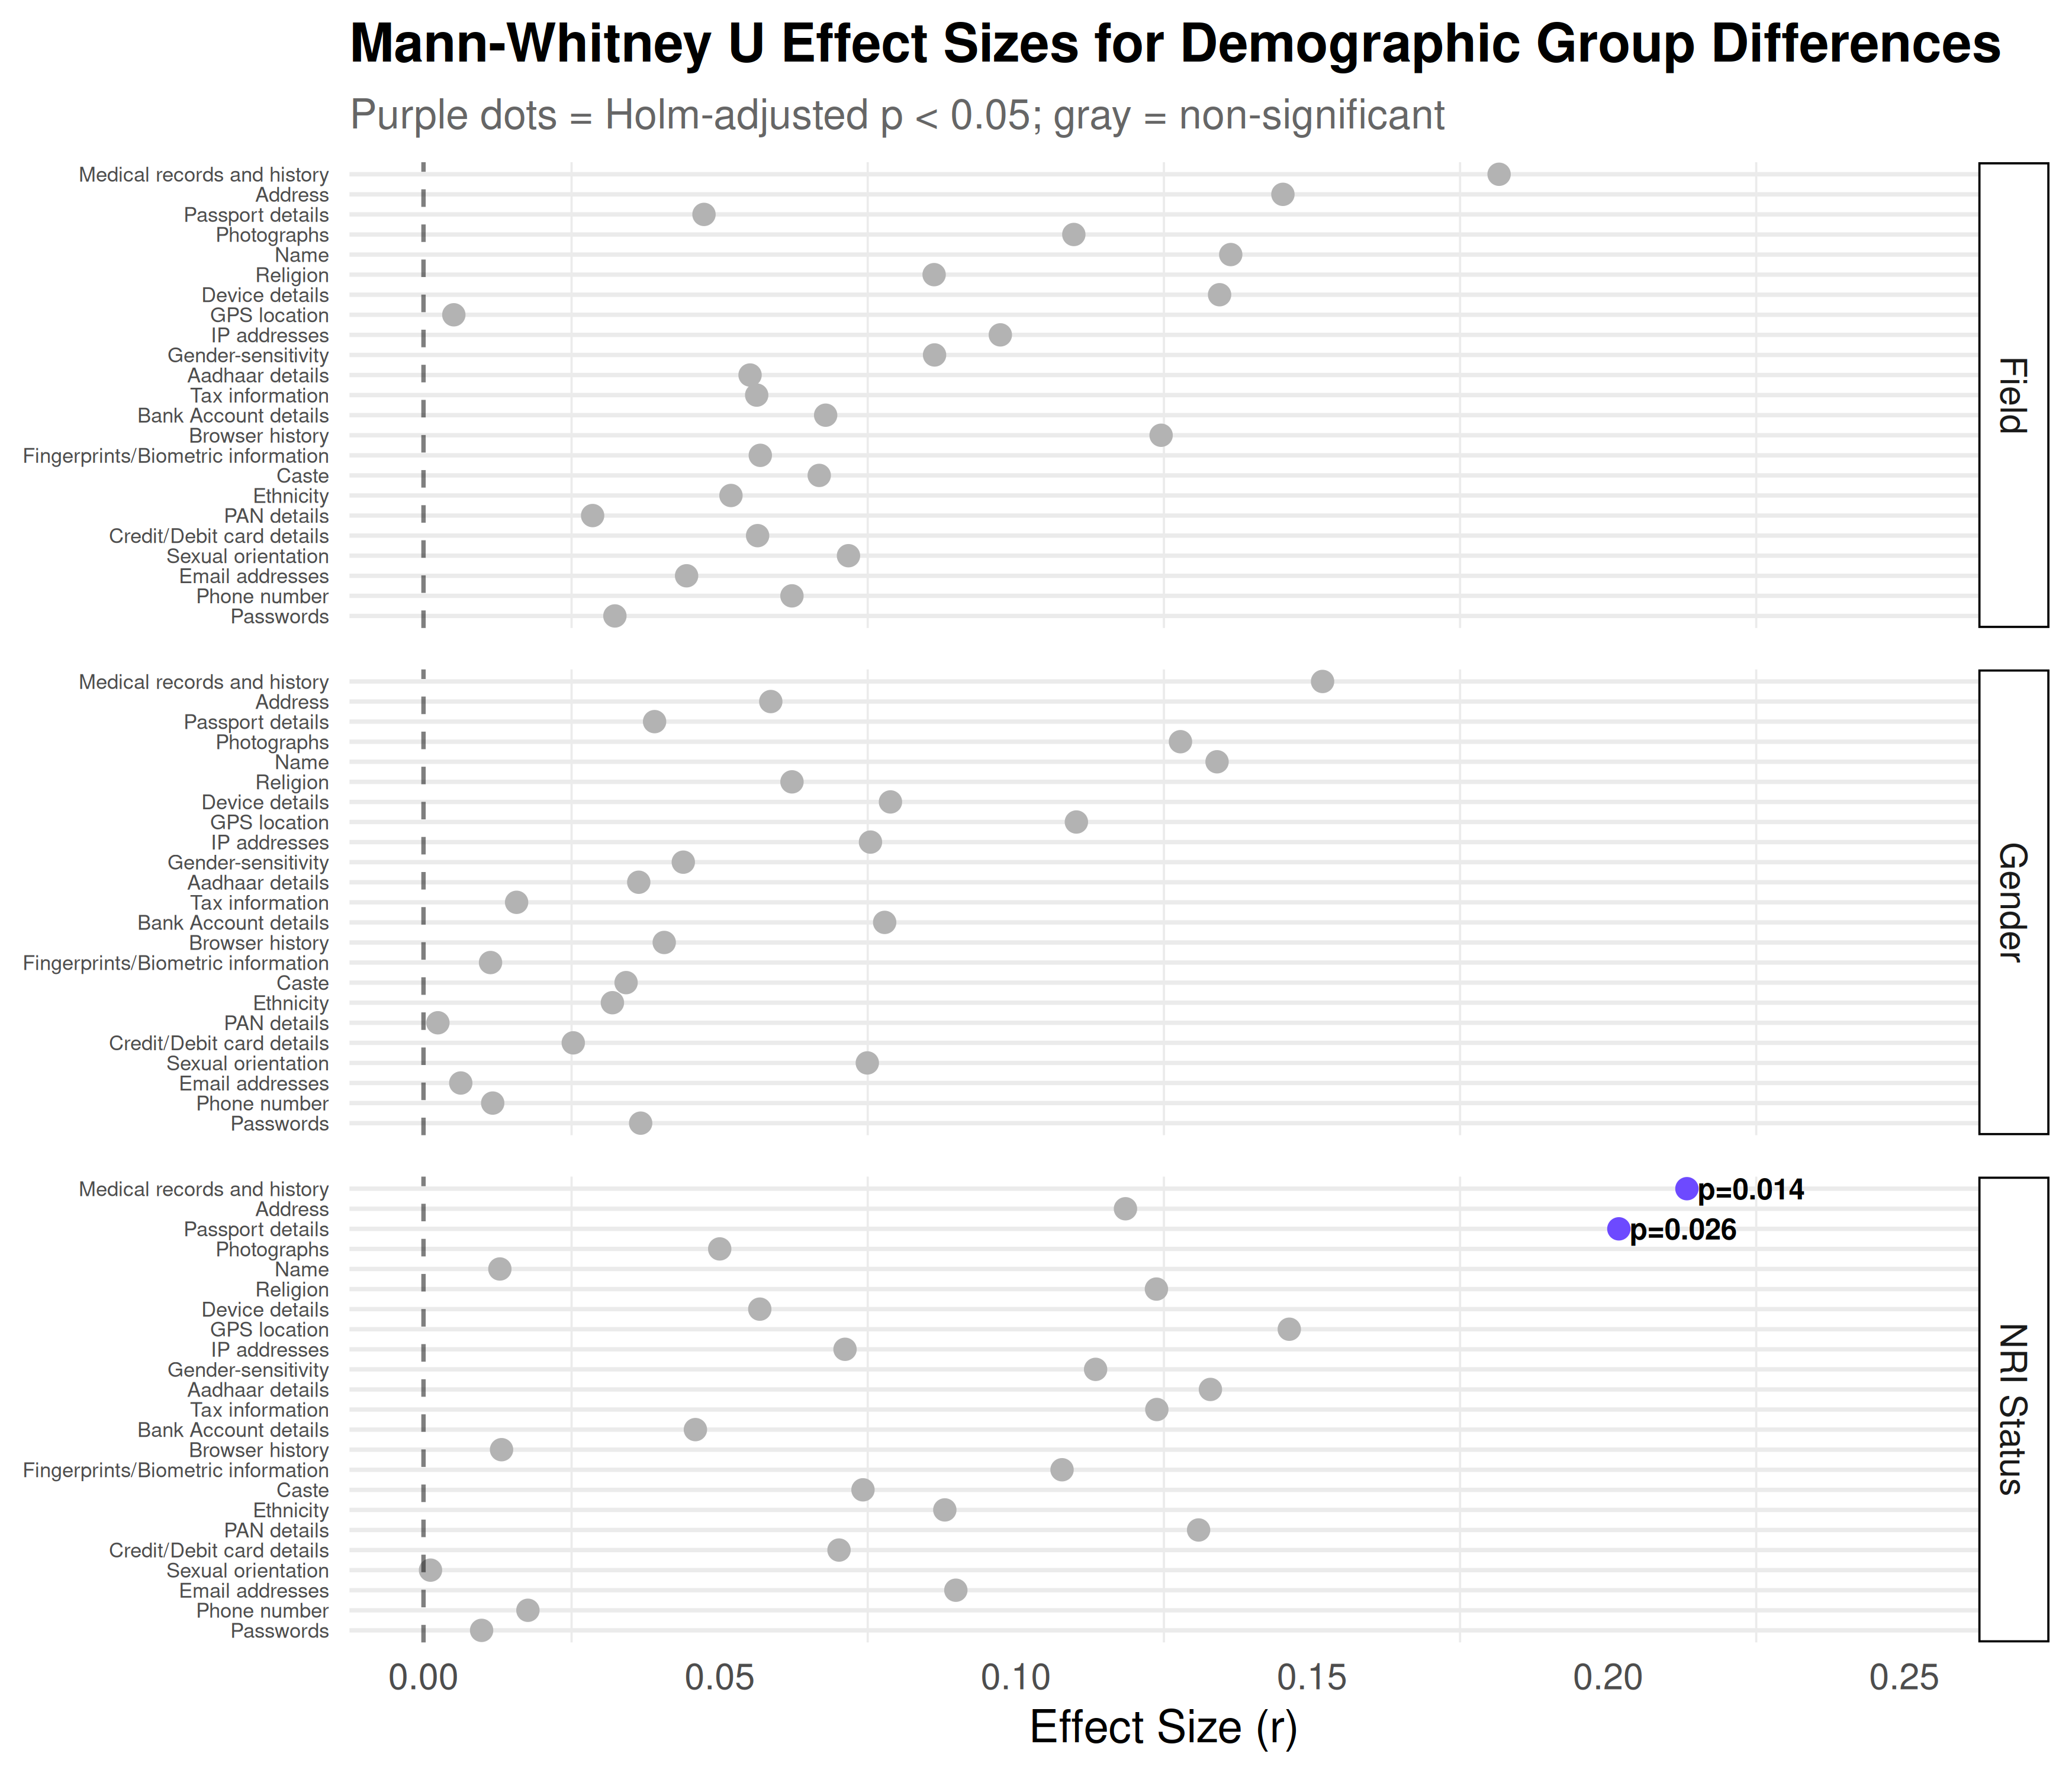
\includegraphics[width=1.0\linewidth]{Plots/Sensitivity_Mann_Whitney_U.png}
    \caption{Mann-Whitney U effect sizes (r) and Holm-adjusted p-values across 22 data sensitivity categories and 3 demographic predictors. Purple dots indicate statistical significance after Holm correction (p\_holm < 0.05); numerical labels show exact p\_holm values for significant findings. Gray dots represent non-significant effect sizes. Only NRI field with passport details (p\_holm = 0.026, r = 0.20) \& Medical records and history(p\_holm = 0.014, r = 0.21) achieve statistical significance. All effect sizes remain below Cohen's medium threshold (r = 0.30)}
    \label{fig:Sensitivity MWU}
\end{figure}

Similarly, the variance of \textit{Gender} and \textit{Field of work} on the \textit{perceived control} value for each respondent was measured using Mann Whitney U tests as well. In line with the prior comparison to sensitivity, both the demographics yielded no statistically significant effect with p = 0.117 and p = 0.296 respectively \ref{fig:Perceived control MWU}. Linear regression model was estimated to understand the isolated effects on this aggregate value, however, none of them achieved statistical significance (p > 0.12). Both the regression plots are provided in the Appendix for reference purposes.

\begin{figure}
    \centering
    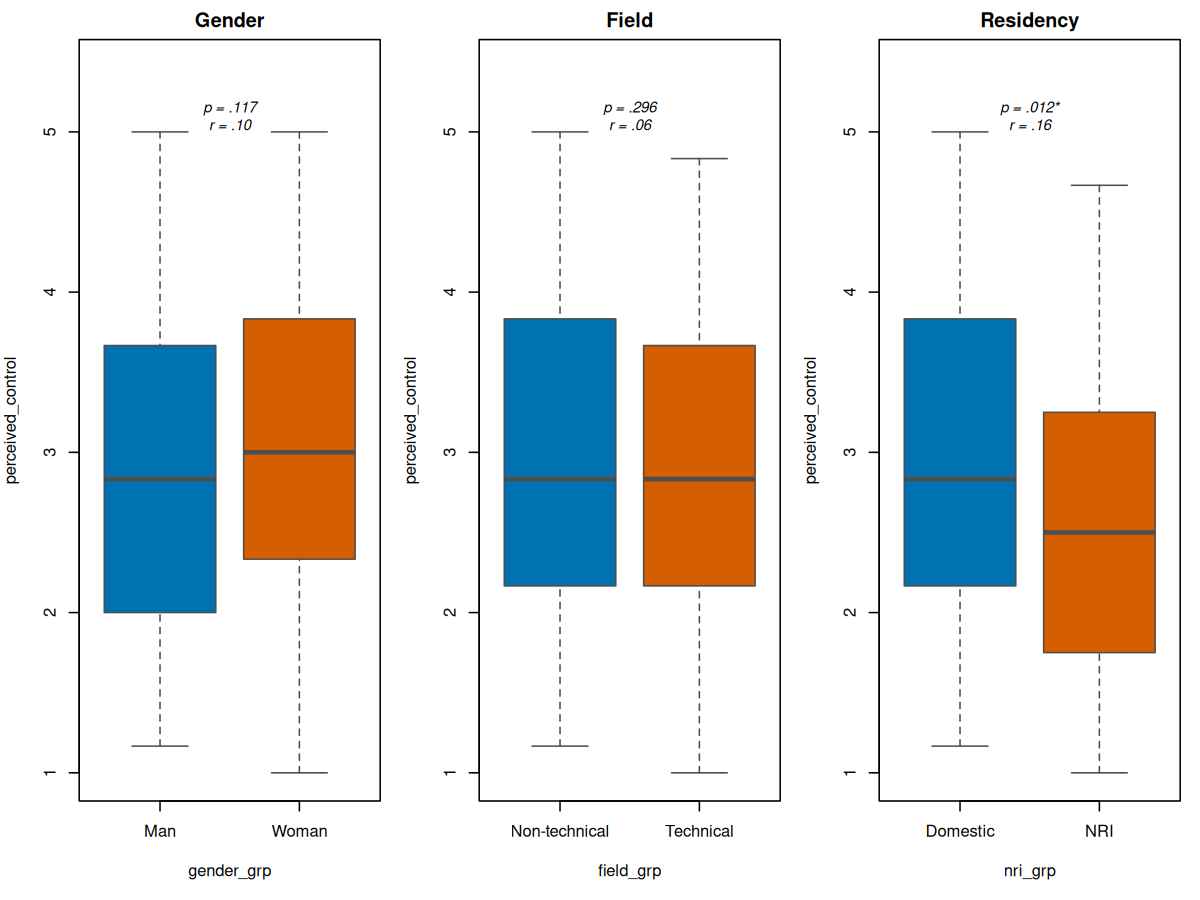
\includegraphics[width=1.0\linewidth]{Plots/Perceived_control_MWU.png}
    \caption{Mann-Whitney U tests revealed no significant differences by gender (p = 0.117, r = 0.10) or field of work (p = 0.296, r = 0.06). The NRI comparison yielded a statistically significant difference (p = 0.012, r = 0.16), with domestic respondents reporting higher perceived control than NRI respondents}
    \label{fig:Perceived control MWU}
\end{figure}


\section{Qualitative Analysis} \label{Sec: Qual Analysis}

As discussed in \ref{Subsec: control}, the participants could elaborate on their choices regarding perceived control over personal data processing through optional open-text fields. These were included to capture the nuances arising from this sensitive yet necessary discourse. Post data collection, approximately 100+ responses per item were obtained, with considerable variation in response length and depth. Additionally, the open-text question regarding the Personal Data definition \ref{Subsec: IUIPC} also yielded diverse answers covering various interpretations of constitutes personal data. Upon initial familiarization, many responses demonstrated substantive nuance across multiple topics within this domain. This richness informed the decision to employ Reflexive Thematic Analysis (RTA) for deeper interpretation and theme construction. 

\subsection{Reflexive Thematic Analysis} \label{subsec: Reflexive TA}

Given the researcher's interpretive role throughout the research process in terms of assumptions, from shaping the survey design to theme development during analysis, Reflexive Thematic Analysis aligned with the epistemological commitment to foreground subjectivity as an analytic resource rather than treating it as bias \cite{braun_using_2006, braun_reflecting_2019}. Reflexive TA offers the methodological flexibility that requires the researcher to iteratively think and understand what they're working with, therefore helping their own perspective change and evolve with each iteration. This flexibility combined with the structured six-stage analytic process provides a comprehensive way to understand the patterns within the data and construct themes from them. These six stages are: 
\begin{enumerate}
    \item Familiarizing yourself with your data
    \item Generating initial codes
    \item Searching for themes
    \item Reviewing themes
    \item Defining and naming themes
    \item Producing the report
\end{enumerate}

Other methods like Content Analysis or Codebook TA offered methodological rigor similar to Reflexive TA. However, they compromise in terms of accounting for the positionality of the researcher and how it usually impacts analysis. In contrast, this method preserves such nuance while also ensuring that the responses of the participants are not forced into pre-defined categories. 

Additionally, my positionality as a Non-Resident Indian, who resided in the country till the completion of my Bachelor's degree influenced the way I initially understood the context and narrative around the conversation of personal data privacy from a Global South perspective, where the norm for privacy is often from a shared perspective \cite{sambasivan_privacy_nodate}. Furthermore, the lack of awareness around legal jargon creates an atmosphere where the system often offloads the burden of being informed and knowledgeable to the user, thereby forcing them to choose their convenience over privacy. This reflexive thought process was employed during all the phases of conducting this research and is visible in the theme development as well. However, any assumptions made implicitly were documented through memos to maintain provenance.     

\subsection{Analytic Process} \label{subsec:qual analysis}

In order to stay true to Braun and Clarke's approach, the responses for these six control items and the personal data definition were read through twice in a thorough manner to obtain \textbf{familiarity with the data}. Approximately, this consisted of around $\sim$ 800 open-text responses, annotating information that was caught on first glance. Using Atlas.ti, these responses were then sorted and \textbf{coded together initially}, since it was observed that they had many recurring narratives that repeated across items. This process resulted in the generation of 72 codes on the first pass. These codes, along with the reasoning for assigning some of them in a certain manner was noted for accuracy purposes. Additionally, they were also discussed with my supervisors, who have between them have a strong foundational experience of using Reflexive TA. Upon receiving feedback, the codes were revisited individually and either re-worded or even recoded from scratch where necessary. This process ensure the rigor was maintained throughout the coding phase, without losing the nuance mentioned by the participants. This second pass of coding resulted in the generation of 119 codes. 

These set of codes were then sorted into a Miro board for having a broader overview of all the existing information, to help sort it better. In the \textbf{search for suitable themes}, the codes were gathered and sorted together based on their relevancy to the plausible themes that were identified within these codes. The themes were then reviewed against the initial codes and their respective quotations, helping to triangulate this entire process. Each of the identified themes and their subsequent sub-themes were then explicitly \textbf{defined and named} in terms of their scope. These themes and sub-themes were then extensively discussed with my supervisors to ensure clarity and soundness in their alignment. Finally, the entire process was cross-checked, along with the selection of certain relevant quotes for each code and documenting the choices that were made to ensure a sound analytic procedure. 

Two LLM-generated responses were ear-marked under the code ``LLM response'' and omitted from any form of thematic analysis, to ensure the perspectives were kept human and their quality maintained. Similarly, responses which were in plain binary agreement or disagreement across all the questions were marked separately but left out of theme building since they do not contribute in a meaningful way. Responses (n=8) which were repeated by the same users across multiple questions, were only considered once while the rest were marked as duplicate and omitted. Finally, responses like `No reason', `Same as before', `NA' and repetition of the question statement were also marked and omitted since they do not contribute to the quality of the analysis in a meaningful manner. 

Since the personal data question required the users to name some items which they think falls into this category, such list of items mentioned across each response was marked as a bucket code to ensure the nuance present in the rest of the response wasn't lost and the codebook was not filled up with just names of the various personal data items. Since this bucket code was present for every response of the personal data question, it is considered as a supportive pillar while creating the theme around these codes.

\subsection{Themes} \label{subsec: themes}

Upon segregation, there are 4 themes which have been identified from the responses of the users, with each having sub-themes to further explain the various nuanced perspectives. The consolidated list of all the themes and their sub-themes along with a brief explanation and example quotations is as follows:

\begin{enumerate}
    \item \textbf{What makes `Data' personal?}: \textit{This theme focuses on the user definition of their Personal data, how they use and create such data along with their explanation of how must it be used or accessed by others}
    \begin{enumerate}
        \item \textbf{Identity focused information}: Sub-theme primarily captures the interdependence of user with their identity, along with the intricacy of understanding person - data relationship. In relation to this, users also point out that this identification can be both direct or indirect in its nature, while such data always needing or having privacy and security
        \begin{quote}
            ``Any data that represents my identity or belong to me''
        \end{quote}
        \begin{quote}
            ``Any personally identifiable information, including health information that can trace me or my family's identity''
        \end{quote}
        \item \textbf{User-originated attributes}: This sub-theme explains the users opinions on how data is basically something they generate hence describing them uniquely. Due to such uniqueness, some users also claim that the companies use this data to build a digital profile of their identity of tracking or advertising purposes
        \begin{quote}
            ``Anything which gives away any key unique trait/identification/interests of mine''
        \end{quote}\
        \begin{quote}
            ``Any data generated by me that can be used to influence my behaviour''
        \end{quote}
        \item \textbf{Information exclusivity}: Focus on the importance of users' consent, their perspectives about not sharing such data with anyone and selective access. In a slight contradiction, some users also talk about their willingness to share such data with others, with the caveat of their choice still being present nonetheless
        \begin{quote}
            ``Its a confidental data which shouldn't be visible to others without the owner consent.''
        \end{quote}
        \begin{quote}
            ``Anything that belongs to me is personal. Until I deliberately choose it to be public.''
        \end{quote}
    \end{enumerate}
    
    \item \textbf{Deficits in privacy agency and awareness}: \textit{This theme discusses about user pitfalls with respect to processing practices including their lack of awareness about such practices while not having sufficient information being provided by the companies which reduces transparency. All this leads to the users showcasing mixed feelings of overall trust, primarily leaning towards corporate distrust} \label{theme:T2}
    \begin{enumerate}
        \item \textbf{Agency constraints and powerlessness}: This sub-themes deals with the various the fears of the users in terms of their social standing against the companies stemming from confusion, data misuse, presence of AI, and lack of choice and control. While some users echo their right to have control over data, a few also contradict by talking about their existing control and how this benefits them due to the personalized content. Many of the users also recollect their personal experiences of advertising and data malpractices which lead to possible cyber crimes
        \begin{quote}
            ``Generally I get recommendations and I don't know how they know it''
        \end{quote}
        \begin{quote}
             ``I didn't want to become victim of cyber crime , abuse because of my opinions , don't want them to track my movements, calls me on birthday and asking for donations , morphing photos , getting loans my using my details.''
        \end{quote}
        \begin{quote}
             ``I didn't want to become victim of cyber crime , abuse because of my opinions , don't want them to track my movements, calls me on birthday and asking for donations , morphing photos , getting loans my using my details.''
        \end{quote}
        \item \textbf{Process transparency and information access}: Describes the plight of users about their awareness and knowledge gaps, denial of information, and lack of transparency about these processes by the companies. Few users however do talk about consent revocation specifically being quick and easy, especially due to their usage of automated tools
        \begin{quote}
            ``If there are multiple stakeholders who own/share access to the data, the removal process is complex and could have mistakes''
        \end{quote}
        \begin{quote}
            ``Not that at all easy, first not much awareness that one can withdraw and also not easy to find the procedure to withdraw''
        \end{quote}
        \begin{quote}
            ``In the past, I have requested my personal data to be deleted with my account when I no longer use the service (ex: food delivery apps, job application sites). The process gas been quick and simple.''
        \end{quote}
        \item \textbf{Post-hoc confirmation challenges}: Deals with users talking about not receiving any valid and believable confirmation primarily related to their consent withdrawal and deletion of their data. Claims of an illusion of deletion being created by the companies are made mainly because the data will always exist on the cloud and their servers
        \begin{quote}
            ``There are features to whitdraw but I don’t know if they actually do it or not''
        \end{quote}
        \begin{quote}    
            ``Because I am not sure that if they comply and remove my data, what if it has already been stored in third party servers and cannot be erased from there.''
        \end{quote}
        \item \textbf{Contingent trust}: This sub-theme focuses on the conditionality of user's trust about these processes and more importantly about the companies. Some of the users however, explicitly talk about them making decisions on their own, which often leads to them conditionally trusting the companies and their process.
        \begin{quote}
            ``I think companies hide a lot behind their fine print on how they use and process data and I'm not fully informed''
            ``I believe most reputable websites and applications provide privacy notices, consent requests, or terms and conditions explaining how my personal data will be collected and processed. I make an effort to review these notices, especially when sharing sensitive information, although I understand that the level of detail and transparency may vary between organizations.''
        \end{quote}
    \end{enumerate}
    
    \item \textbf{Corporate opacity and accountability gaps}: \textit{This theme describes the various practices by the companies which are aimed to deceive the user and the law in order to make profits. Furthermore users also talk about companies and their influence peddling to ensure non-compliance}
    \begin{enumerate}
        \item \textbf{Asymmetric information disclosure}: This sub-theme describes the users perceptions about information non-disclosure by the companies in addition to their unconsenting data processing practices. Some users do claim that while they are fully informed by the companies in their privacy policies, they are still skeptical about valid implementation
        \begin{quote}
            ``I get a disclaimer that my data is going to be used but i don't get a reason or justification as to where it is being used and when''
        \end{quote}
        \begin{quote}
            ``Even though there are disclaimers on the data usage, there is no mechanism to know if it is followed.''
        \end{quote}
        \item \textbf{Manipulative design}: Dark patterns described by the users which are employed by these companies with the intent to misguide, often also resulting in the users skipping the documentation
        \begin{quote}
            ``Companies usually make it super hard to withdraw consent by hiding/fine printing info as to how to go about it so users lose interest''
        \end{quote}
        \begin{quote}
            ``Signup is often one click but try deleteing any account and count your number of clicks'' 
        \end{quote}
        \item \textbf{Corporate evasion and greed}: Users discuss the ways companies evade legal compliance, stemming from their lack of accountability and their monetary end-goals. They extensively discuss psuedo-compliance using real-world instances of such situations
        \begin{quote}
            ``It is not beneficial for companies,to alert the customer,as usually people don't trust multi national conglomerates, so they do legally so but in a way,that people don't immediately grasp the importance and just give in, without going through all that information...I hold the notion of personal marketting to lowest esteem, because it makes me feel constantly perceived,and gives an air of declining privacy of mine''
        \end{quote}
        \begin{quote}
            ``Aadhar details of 800million people got leaked. Who really gives a fuck in India. There's no recourse for private leaks as well''
        \end{quote}
        \begin{quote}
            ``Although many companies claim to follow data protection laws, I am not always confident that they fully comply with them in practice. News reports about data breaches, privacy concerns, and the misuse of personal information by large technology companies have made me more cautious. While some organizations likely take these laws seriously, I believe others may focus more on appearing compliant than on consistently protecting users’ personal data. ''
        \end{quote}
    \end{enumerate}

    \item \textbf{Structural Governance shortcomings}: \textit{This theme explores the various hiccups in the legal processes for the users ranging from lack of awareness, procedural hassles not being worth it and primarily, enforcement gaps. Users also hope for a change and improvement in these shortcomings}
    \begin{enumerate}
        \item \textbf{Epistemic legal uncertainty}: This sub-theme deals with conditional awareness, knowledge, and confidence of the users about the various laws. Even the users who claim to have knowledge, mention about their skepticism towards the effectiveness of such laws. However, few users show belief in the existing legal systems, instead expressing doubts on the companies and their compliance
        \begin{quote}
            ``I don't think there's that much awareness Laws don't get implemented so easily''
        \end{quote}
        \begin{quote}
            ``There are obviously laws but I dont know the effectiveness since laws vary from country to country and an individual cant know laws of all the various countries and it often do happens you data is sold not only within your country but also out of the country to various data brokers.''
        \end{quote}
        \item \textbf{Enforcement barriers}: Conditionality is further extended towards the distrust in the enforcement procedures either due to organizational noncompliance or lack of transparency. Users believe that the hassles involved in fighting against these giant corporations only amplifies their distrust on both the companies and the legal procedure itself
        \begin{quote}
            ``I believe many organizations strive to comply with data protection laws, but the level of compliance can vary depending on the organization's size, industry, and commitment to privacy. Without transparency or independent verification, it is difficult to be certain.''
        \end{quote}
        \begin{quote}
            ``I believe legislation still needs to catch up to the developments and practices of tech companies. Also, legal recourse for an average member of the public can be prohibitively expensive in a country where justice is not always delivered in a timely manner.''
        \end{quote}
        \item \textbf{Wishful reforms}: Users acknowledge the need for better legal procedures, increased awareness and improvement in the overall legal implementation
        \begin{quote}
            ``Enforcement in a defined timeline is a must which I feel we are lacking''
        \end{quote}
        \begin{quote}
            ``Even if there are, people are not aware of such laws. People should be educated in such laws''
        \end{quote}
    \end{enumerate}
\end{enumerate}

The overlap between these themes, especially how despite high sensitivity perceptions, corporate opacity contributes to agency deficits within the context of regulatory permissiveness, is explored as interconnected pathways in Section \ref{chapter:discussion}, alongside the quantitative results to address the research questions \ref{rq:1} \ref{rq:2} in a broader analytical manner. 

\section{Digital Personal Data Protection Act (DPDPA)}\label{sec:DPDPA analysis}

As described in \ref{Subsubsec: DPDPA}, the questions related to this Act comprised of both quantitative and qualitative aspects. Initially, responses were analyzed in a simple descriptive manner by aggregating the number of participants who answered each question as shown in table \ref{tab:dpdpa-awareness}. If the open-text responses were answered for the respective questions, this data was coded and analyzed in simple descriptive summarization manner to ensure the codes stayed as close to the original data as possible. These results and their subsequent descriptive interpretation is discussed further in Section \ref{DPDPA discussion}. 


\begin{table}[htbp]
    \centering
        \begin{tabular}{lr}
            \toprule
            \textbf{Category} & \textbf{n(\%)} \\
            \midrule
            \multicolumn{2}{l}{\textbf{DPDPA Awareness}} \\
            I have heard about it and know its purpose & 54 (21\%) \\
            I have heard about it but do not know anything else & 85 (33\%) \\
            I have not heard about it & 103 (40\%) \\
            Other & 17 (6.6\%) \\
            \cmidrule(l){1-2}
            \multicolumn{2}{l}{\textbf{DPDPA Privacy}} \\
            I am not sure & 22 (41\%) \\
            No & 6 (11\%) \\
            Yes & 26 (48\%) \\
            \bottomrule
        \end{tabular}
    \caption{DPDPA Awareness and Privacy beliefs}
    \label{tab:dpdpa-awareness}
\end{table}

